\chapter{Implementierung}\label{ch:implementierung}
Das Projekt wurde in C++11 umgesetzt. Für die Erstellung einer Benutzeroberfläche wurde die QT5 Bibliothek verwendet \cite{qt5}.
Für verschiedene Algorithmen aus der Mustererkennung wurde die OpenCV2 Bibliothek genutzt \cite{opencv}. Außerdem verwenden wir CMake
als plattformunabhängiges Build-System \cite{cmake}. Für das Projekt haben wir zwei separate Anwendungen erstellt, den QViewer und das Auto-Train
Programm.

\section{QViewer}
Der QViewer ermöglicht uns die Visualisierung der Eingabedaten. Nachdem die Landmark und Action Unit Dateien geladen wurden,
kann der Nutzer eines der Videos auswählen und abspielen. Zu jedem Frame zeigt
der QViewer welche Action Units mit welcher Ausprägung aktiv sind (vgl. \cref{Implementierung.QViewer}).

\begin{figure}
\begin{center}
\includegraphics[width=0.75\textwidth]{qviewer.png}
\caption{Screenshot der QViewer Anwendung}
\end{center}
\label{Implementierung.QViewer}
\end{figure}


\section{Auto-Train}
Wie bereits in Kapitel 2 erwähnt, ist ein guter Klassifikator abhängig von der Wahl verschiedener Variablen, wie zum Beispiel
von der Auswahl der Features oder von den Parametern mit denen der Klassifikator trainiert wird.
Das Auto-Train Programm ermöglicht uns, automatisch verschiedene dieser Variablen auszuwählen, basierend darauf ein Klassifikator
zu trainieren und an dem Validierungsset zu evaluieren. Die Resultate der Evaluation werden ebenfalls automatisch gespeichert.
Die Konfiguration, das heisst eine Auswahl der Variablen die miteinander getestet werden sollen, kann aus einer einfach Json-Datei
geladen werden (vgl. \ref{Anhang.config}).

\subsubsection{Feature-Extractor}
Um möglichst viele Kombinationen von einzelnen Features miteinander kombinieren zu können, haben wir eine Feature-Extractor Aggregat
Klasse erstellt, die es uns ermöglicht verschiedene Feature-Extractor aneinander zu koppeln und so kombinierte Features zu extrahieren.
Kombiniert man beispielsweise die Extraktion der Orientierung zum Mittelpunkt, zusammen mit der Distanz zum Mittelpunkt, so erhält man
pro Landmark zwei Features und damit pro Frame einen 132 elementigen Feature-Vektor \ref{Implementierung.Feature-Extractor}.\newline

\begin{figure}
\begin{center}
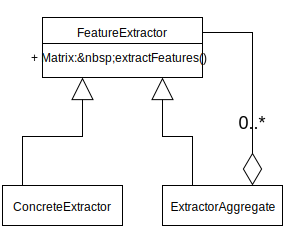
\includegraphics[width=0.4\textwidth]{feature_extractor.png}
\caption{UML-Diagramm der Feature-Extractor Klasse}
\end{center}
\label{Implementierung.Feature-Extractor}
\end{figure}



% \begin{itemize}
%   \item Zum trainieren und evaluieren
%   \item Kurzes Wort zum Design von FeatureExtractor
%   \item Automatisches Speichern aller relevanten Dateien.
%   \item Erwähnung der JSON-Konfigurations-Datei
%     \begin{itemize}
%     \item Design von Processors
%   \end{itemize}
% \end{itemize}

%%% Local Variables:
%%% mode: latex
%%% TeX-master: "../../paper"
%%% End: